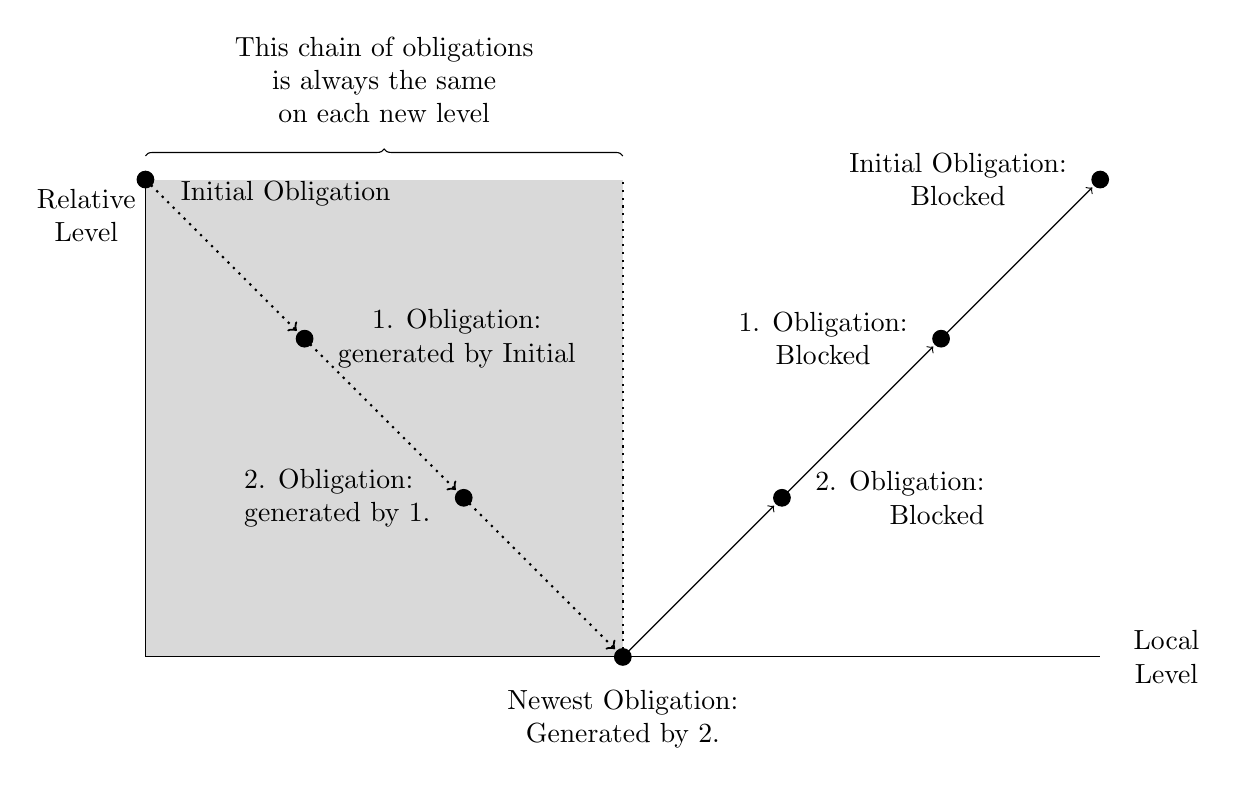
\begin{tikzpicture}[]


\fill[black!15!white] (0,0) -- (0,\textwidth/2) -- (\textwidth/2,\textwidth/2) -- (\textwidth/2, 0) -- cycle;


% horizontal axis
\draw[-] (0,0) -- (\textwidth,0) node[align=center, right=3mm] {Local \\ Level};


%1.
\filldraw (0,\textwidth/2) circle (3pt) node[align=right, below right, label={[xshift=2mm, yshift=1mm, below right]Initial Obligation}] {};

%connection 1. and 2.
\draw [thick, dotted, ->]
(0,\textwidth/2) --(\textwidth/6 - 1mm,\textwidth/3 + 1mm);

%2.
\filldraw (\textwidth/6,\textwidth/3) circle (3pt) node[align=center,   right=3mm] {1. Obligation: \\ generated by Initial};

%connection 2. and 3.
\draw [thick, dotted, ->]
(\textwidth/6,\textwidth/3) --(\textwidth/3 - 1mm,\textwidth/6 + 1mm);

%3.
\filldraw (\textwidth/3,\textwidth/6) circle (3pt) node[align=left,   left=3mm] {2. Obligation: \\ generated by 1.};

%connection 3. and 4.
\draw [thick, dotted, ->]
(\textwidth/3,\textwidth/6) --(\textwidth/2 - 1mm,0 + 1mm);

%4.
\filldraw (\textwidth/2,0) circle (3pt) node[align=center,   below=3mm] {Newest Obligation: \\ Generated by 2.};

%4 and 3'
\draw [->]
(\textwidth/2,0 ) -- (\textwidth - \textwidth/3 - 1mm,\textwidth/6 - 1mm);

%3.'
\filldraw (\textwidth - \textwidth/3,\textwidth/6) circle (3pt) node[align=right,   right=3mm] {2. Obligation: \\ Blocked};


%3' and 2'
\draw [->]
(\textwidth - \textwidth/3, \textwidth/6 ) -- (\textwidth - \textwidth/6 - 1mm,\textwidth/3 - 1mm);


%2.'
\filldraw (\textwidth - \textwidth/6,\textwidth/3) circle (3pt) node[align=center, left=3mm] {1. Obligation: \\ Blocked};


%connection 2.' and 1.'
\draw [->]
(\textwidth - \textwidth/6,\textwidth/3) -- (\textwidth - 1mm,\textwidth/2 - 1mm);


%1.'
\filldraw (\textwidth,\textwidth/2) circle (3pt) node[align=center,   left=3mm] {Initial Obligation: \\ Blocked};


% ranges
%\draw	(1,3.5) node{{\scriptsize Constant flux}};
%		(4,3.5) node{{\scriptsize Field weakening}};

\draw[thick, dotted] (\textwidth/2,0) -- (\textwidth/2,\textwidth/2) node[] {};



% Vertical axis
\draw[] (0,0) -- (0,\textwidth/2) node[align=center, below left] {Relative \\ Level};
% \draw[] (\textwidth,0) -- (\textwidth,\textwidth/2) node[left=5mm] {};

\draw [decorate, decoration={brace, mirror}] (\textwidth/2, \textwidth/2 + 3mm) -- node[above=3mm, align=center]{This chain of obligations \\ is always the same \\ on each new level} (0, \textwidth/2 + 3mm);



\end{tikzpicture}